\chapter{Ergebnisse}\label{ch:ergebnisse}
\begin{figure}[H]
    \begin{center}
        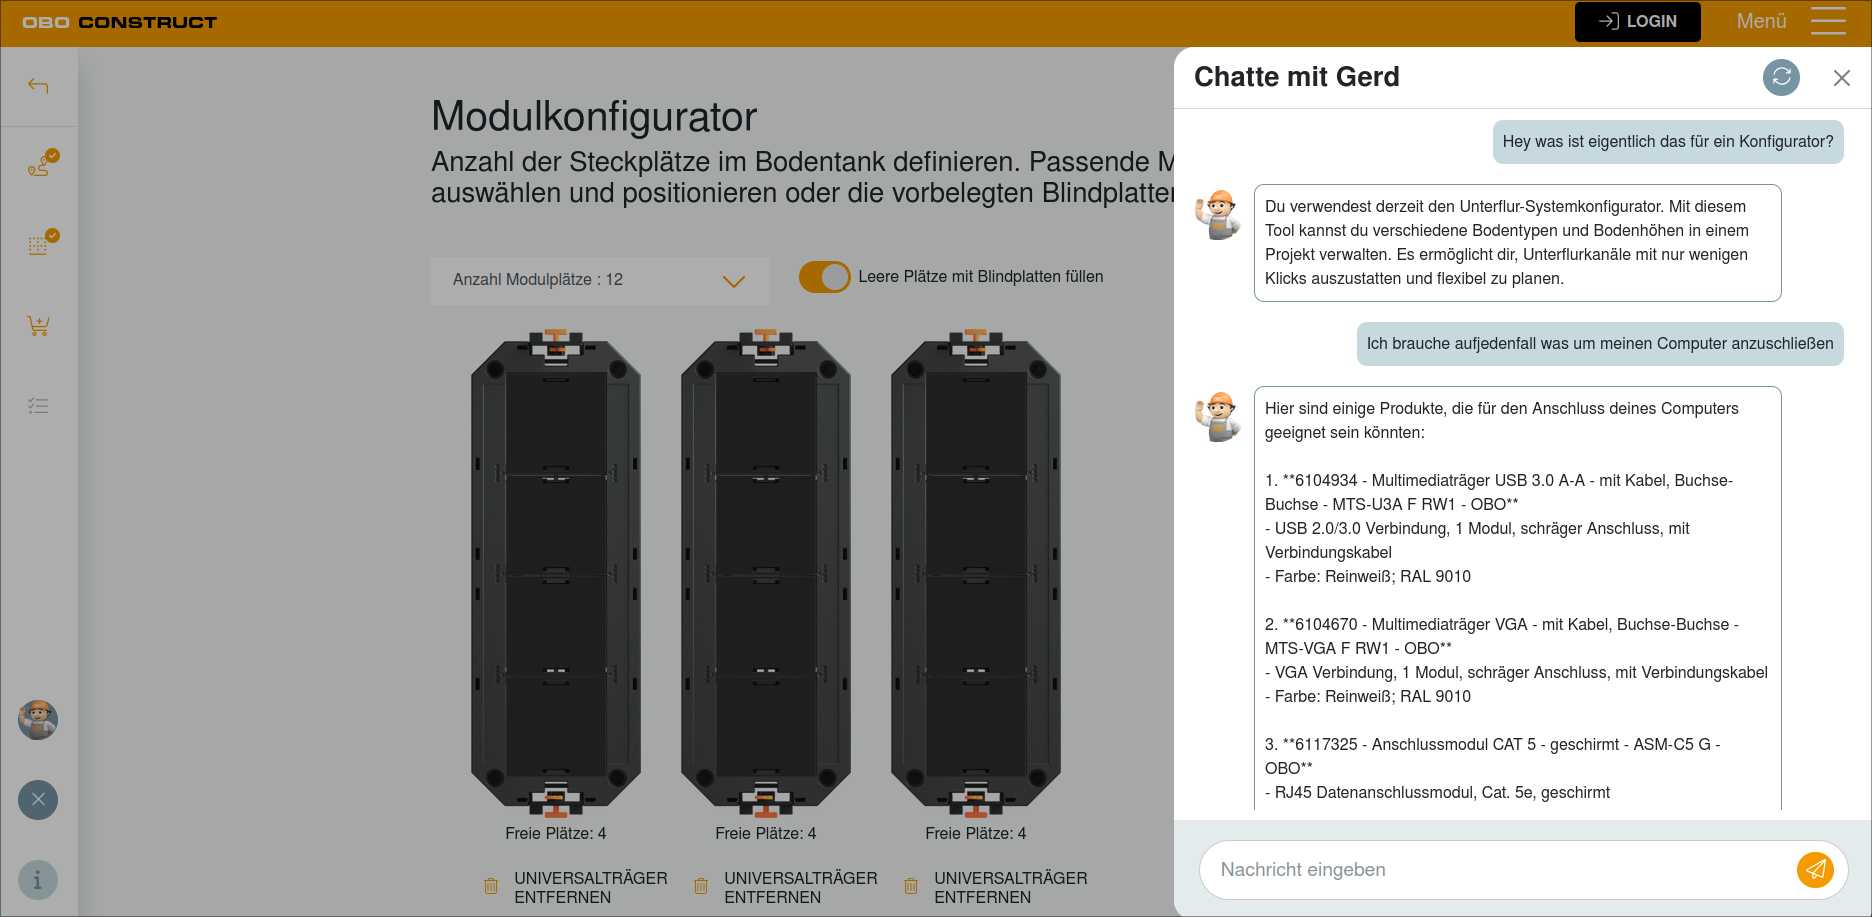
\includegraphics[width=14cm]{bilder/chatbot.png}
        \caption{Screenshot der Anwendung mit geöffnetem Chatbot}\label{fig:bodentank}
    \end{center}
\end{figure}
Zu sehen ist ein Screenshot des Unterflur-Konfigurators mit geöffnetem Chatbot.  
Der Chatbot ist am rechten Rand platziert und kann durch Klicken auf das Chatbot-Symbol (unten links) geöffnet werden.\\  
Zudem ist auch die Kernfunktionalität des Chatbots zu sehen. Passend zur Anfrage des Nutzers erhält der Chatbot Produktdaten aus der  
Vektor-Datenbank und gibt diese bei Bedarf dem Nutzer aus oder geht auf die Inhalte ein.  
Hier sieht man, wie das Embedding-Modell und die Suche in der Vektor-Datenbank den Begriff \enquote{Computer} mit Produkten über USB, VGA und CAT 5  
assoziieren konnten.\\  
Dazu hat die \gls{llm} verstanden, dass diese Produkte gebraucht werden können, um Verbindungen diverser Art zu einem Computer herzustellen  
und für die Anforderungen eines Unterflursystems, wie der Nutzer es beschrieben hat, passend sein könnten.\\  
Auch wenn das Projekt eindeutig umfangreicher geworden ist, als ursprünglich von mir angenommen, bin ich sehr zufrieden mit dem Ergebnis.  
Die Präsentation des Chatbots vor dem Kunden steht noch aus, aber bisher habe ich von Arbeitskollegen positives Feedback erhalten  
und bin zuversichtlich, dass der Chatbot auch dem Kunden gefallen wird.\\\\  
Zum jetzigen Zeitpunkt stehen noch kleinere Anpassungen an, bevor der Chatbot in die Produktion gehen kann. Ich bin jedoch zuversichtlich,  
dass ich diese in der nächsten Zeit noch umsetzen kann und der Chatbot dann produktiv genutzt werden kann.  
Danach wird sich zeigen, wie der Chatbot bei dem Kunden und den Nutzern ankommen wird und ob wir den Chatbot auch auf weitere Konfiguratoren  
des Kunden erweitern werden.